%!TEX root = ../bgsu21.tex

\begin{frame}[t]{Beyond the even prime}

	\pause

	Extending the diagonal to a full \textcolor{pblue}{$E_\infty$-coalgebra} structure on chains.

	\smallskip\pause

	These provide an algebraic model for the homotopy theory of spaces.\\ e.g. over $\mathbb Q$ (Quillen--Sullivan) over $\overline{\mathbb F}_p$ (Mandell).

	\smallskip\pause

	\begin{theorem}[Med.]
		The collection of maps $\gchains(\gsimplex^n) \to \gchains(\gsimplex^n)^{\otimes r}$ obtained from compositions of
		\begin{align*}
		\Delta &\colon \gchains(\gsimplex^n) \to \gchains(\gsimplex^n)^{\otimes 2}
		\qquad \text{(AW diagonal)} \\
		\ast &\colon \gchains(\gsimplex^n)^{\otimes 2} \to \gchains(\gsimplex^n)
		\qquad \text{(Join map)}
		\end{align*}
		defines an $E_\infty$-coalgebra on simplicial chains.
	\end{theorem}

	\pause

	\only<5>{\qquad \qquad \scalebox{0.7}{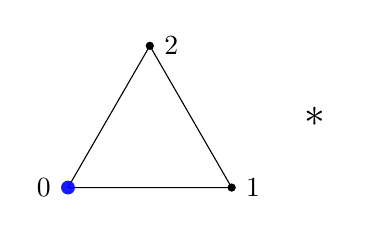
\begin{tikzpicture}[scale=.6]
\coordinate (A) at (210:2);
\coordinate (B) at (-30:2);
\coordinate (C) at (90:2);

\draw[draw=black] (A) -- (B) -- (C) -- (A);

\node[circle,fill=blue, opacity=.9, inner sep=0pt,minimum size=5pt, label=left:{0}] (a) at (A) {};
\node[circle,fill=black,inner sep=0pt,minimum size=3pt, label=right:{$1$}] (a) at (B) {};
\node[circle,fill=black,inner sep=0pt,minimum size=3pt, label=right:{$2$}] (a) at (C) {};

\node[scale=1.5] at (3.5,0.5) {$\ast$};
\end{tikzpicture}
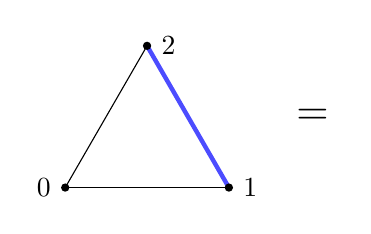
\begin{tikzpicture}[scale=.6]
\coordinate (A) at (210:2);
\coordinate (B) at (-30:2);
\coordinate (C) at (90:2);

\draw[draw=blue,  ultra thick, draw opacity=.7] (B) -- (C);
\draw[draw=black] (C) -- (A);
\draw[draw=black] (A) -- (B);

\node[circle,fill=black,inner sep=0pt,minimum size=3pt, label=left:{$0$}] (a) at (A) {};
\node[circle,fill=black,inner sep=0pt,minimum size=3pt, label=right:{$1$}] (a) at (B) {};
\node[circle,fill=black,inner sep=0pt,minimum size=3pt, label=right:{$2$}] (a) at (C) {};

\node[scale=1.5] at (3.5,.5) {=};
\end{tikzpicture}
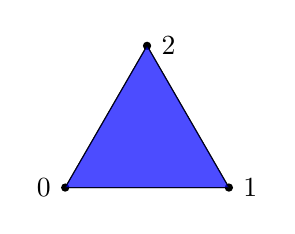
\begin{tikzpicture}[scale=.6]
\coordinate (A) at (210:2);
\coordinate (B) at (-30:2);
\coordinate (C) at (90:2);

\draw[draw=black] (A) -- (B) -- (C) -- (A);

\node[circle,fill=black,inner sep=0pt,minimum size=3pt, label=left:{$0$}] (a) at (A) {};
\node[circle,fill=black,inner sep=0pt,minimum size=3pt, label=right:{$1$}] (a) at (B) {};
\node[circle,fill=black,inner sep=0pt,minimum size=3pt, label=right:{$2$}] (a) at (C) {};

\draw[draw, fill=blue, opacity=.7] (A) -- (B) -- (C) -- (A);
\end{tikzpicture}}}

	\medskip\pause

	\only<6>{Also, versions for: \par
		\qquad \textcolor{pblue}{cubical} (Kaufmann--Med.) and \par
		\qquad \textcolor{pblue}{multisimplicial} (Med.--Pizzi--Salvatore) chains.}
\end{frame}

\begin{frame}[fragile]{Cup-$(p,i)$ structures}

	\vskip-5pt\pause

	\begin{block}{Construction (Kaufmann-Med.)}
		Explicit May--Steenrod structures defining \textcolor{pblue}{operations} on $H^\bullet(-; \Fp)$.
	\end{block}

	\pause

	\begin{block}{Implementation (Med.)}
		In the computer algebra system \verb|ComCH|.
	\end{block}

	\pause

	For example, $\Delta_{3,2}[0,1,2]$ is equal to

	\begin{verbatim}
		- [0,1][0,1,2][0,1] + [0,1,2][0,2][0,1] + [0,2][0,2][0,1,2]
		- [0,1,2][0,1,2][1] - [0,2][0,1,2][1,2] + [0,1,2][1,2][1,2]
		- [0,1][1,2][0,1,2] - [0,1,2][2][0,1,2] - [0][0,1,2][0,1,2]
	\end{verbatim}

	\pause \textcolor{pblue}{Future directions:} \pause
	\begin{enumerate}
		\item Faster implementations for use in TDA. \pause \\
		\item Relation to higher category theory. \pause \\
		\item Cartan and Adem coboundaries. \pause \\
		\item Where are these used in physics?
	\end{enumerate}
\end{frame}